\newcommand{\prompttag}[1]{\textcolor{blue}{\texttt{<|#1|>}}}

\section{Model Training Details}\label{ch2:sec:training}

The final training lineage contains four named models. The pretrained base
model is denoted \textit{Model chk-0}. Supervised fine-tuning (SFT) on
point-in-time evidence-to-analysis pairs produces \textit{Model chk-1}, which
serves as the common parent for two downstream branches. Analysis-to-FOMC-
Minutes-style paragraph-rewriting SFT produces \textit{Model chk-2}; decision
SFT followed by Group Relative
Policy Optimization (GRPO) produces \textit{Model chk-3}. This paper-level
naming maps the experimental Minutes model to \textit{Model chk-2} and the
experimental decision model to \textit{Model chk-3}. Figure~\ref{fig:ch2:training_stage1} summarizes the lineage.

\begin{figure}[htbp]
    \centering
    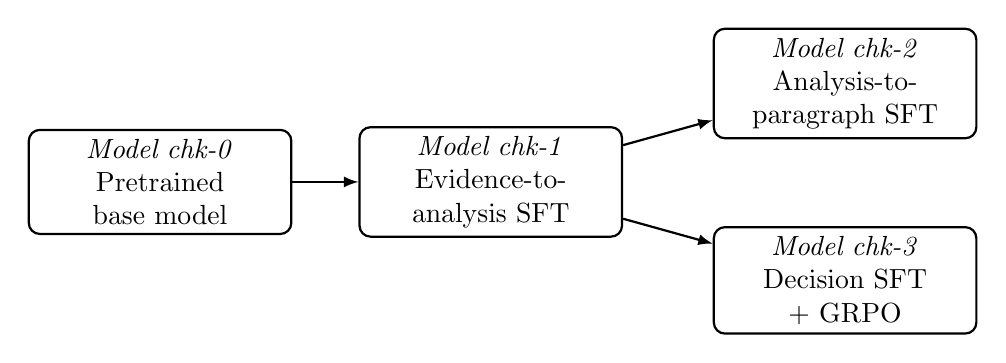
\begin{tikzpicture}[
        >=latex,
        model/.style={draw, rounded corners, align=center, text width=3.1cm,
            minimum height=1.25cm},
        every path/.style={->, thick}
    ]
        \node[model] (chk0) at (0,0)
            {\textit{Model chk-0}\\Pretrained base model};
        \node[model] (chk1) at (4.2,0)
            {\textit{Model chk-1}\\Evidence-to-analysis SFT};
        \node[model] (chk2) at (8.7,1.25)
            {\textit{Model chk-2}\\Analysis-to-paragraph SFT};
        \node[model] (chk3) at (8.7,-1.25)
            {\textit{Model chk-3}\\Decision SFT + GRPO};
        \draw (chk0) -- (chk1);
        \draw (chk1) -- (chk2);
        \draw (chk1) -- (chk3);
    \end{tikzpicture}
    \caption{Final paper-level training lineage.}
    \label{fig:ch2:training_stage1}
\end{figure}

Figure~\ref{fig:ch2:training_process} expands the lineage into the data and
optimization flows for analytical SFT and the two downstream tasks. The
retained diagrams use the original experimental identifiers: the
\textit{Model chk-3} and \textit{Model chk-4} labels printed in the graphics
correspond, respectively, to the paper-level \textit{Model chk-2} and
\textit{Model chk-3}. In addition, the ``Minutes'' box in the decision panel is
an earlier project-side shorthand; the finalized decision model receives the
target-neutral, pre-meeting analysis specified later in this section.

\begin{figure}[H]
    \centering
    \includegraphics[width=\textwidth]{train/stage1.png}
    \par\medskip
    \includegraphics[width=\textwidth]{train/stage2.png}
    \caption{Overview of Two-step Training Process}
    \label{fig:ch2:training_process}
\end{figure}


%SFT
\paragraph*{Supervised fine-tuning.}
SFT adapts the model to the macro-financial tasks by learning from paired
prompts and reference completions. Each training example contains a system
instruction, a user prompt, and a target assistant response. The model is
optimized under teacher forcing, while parameter-efficient adapters reduce
the number of trainable parameters. Figure~\ref{fig:ch2:ft_detail} summarizes
this workflow.


\begin{figure}
    \begin{center}
        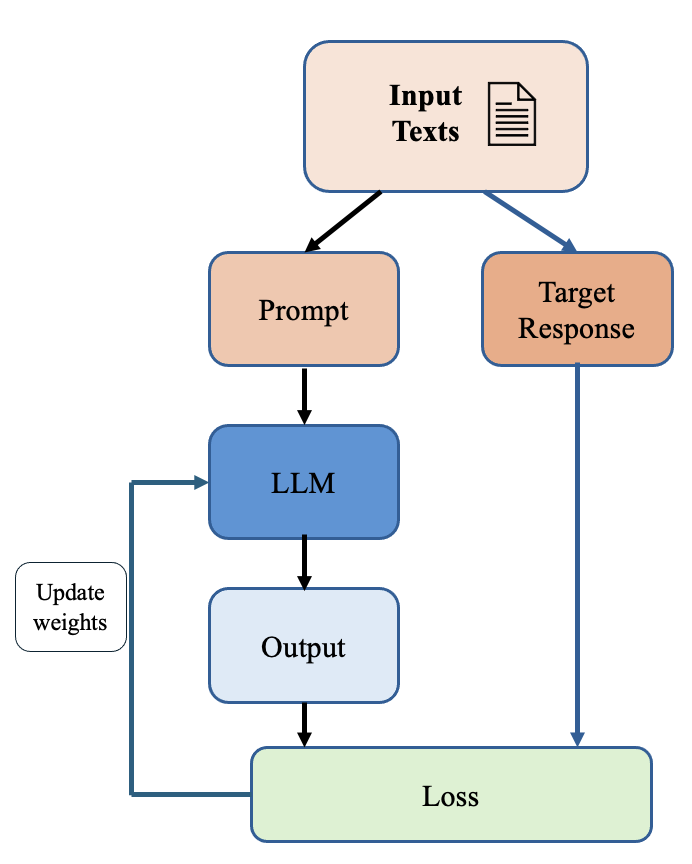
\includegraphics[width=0.3\textwidth]{Chapter2/Chapter2Figs/ft_detail.png}
      \end{center}
      \caption{Supervised fine-tuning workflow.}
      \label{fig:ch2:ft_detail}
\end{figure}



During SFT, let $x=(x_1,\ldots,x_M)$ denote the serialized prompt and
$y=(y_1,\ldots,y_N)$ the target assistant completion. At each target
position, the model predicts a distribution over the vocabulary conditional
on the prompt and preceding target tokens. The mean token-level negative
log-likelihood is
\begin{equation}
    \mathcal{L}_{\mathrm{SFT}}(\theta)
    =
    -\frac{1}{W}
    \sum_{t=1}^{N}
    w_t
    \log \pi_\theta\!\left(y_t\mid x,y_{<t}\right),
    \qquad
    W=\sum_{t=1}^{N}w_t,
\end{equation}
where $w_t\in\{0,1\}$ masks padding and any positions excluded from the
supervised objective. If every completion token is trained, $w_t=1$ and
$W=N$. Thus, SFT minimizes the negative log-probability assigned to the
reference completion; it does not compare a separately decoded response with
the target text.


%RL
\paragraph*{Reinforcement learning.}
Unlike SFT, policy optimization does not require a token-level reference
completion. In the decision task, however, the reference action remains
available to the deterministic reward function: the policy sees the prompt,
whereas the target direction and magnitude are used only to score sampled
completions.

Proximal Policy Optimization (PPO; \cite{schulman2017proximal}) stabilizes
policy-gradient updates by clipping the importance-sampling ratio. Let
$s_t=(q,o_{<t})$ be the token-generation state and define
\begin{equation*}
    \rho_t(\theta)
    =
    \frac{\pi_\theta(o_t\mid s_t)}
         {\pi_{\theta_{\mathrm{old}}}(o_t\mid s_t)}.
\end{equation*}
The clipped policy objective is
\begin{equation}
    \mathcal{J}_{\mathrm{PPO}}(\theta)
    =
    \mathbb{E}_t\!\left[
        \min\!\left(
            \rho_t(\theta)\widehat{A}_t,
            \operatorname{clip}
            \bigl(\rho_t(\theta),1-\epsilon,1+\epsilon\bigr)
            \widehat{A}_t
        \right)
    \right].
\end{equation}
Here, $\widehat{A}_t$ is an advantage estimate rather than the reward itself;
clipping constrains the policy ratio rather than rescaling the reward.




GRPO (\cite{shao2024deepseekmath}) removes the learned value function. For
each prompt $q$, the behavior policy samples a group
$\{o_i\}_{i=1}^{G}$, and the task reward assigns one terminal score
$R_i=R(q,y,o_i)$ to each completion. The group-relative advantage is
\begin{equation}
    \widehat{A}_i
    =
    \begin{cases}
    \displaystyle\frac{R_i-\overline{R}}{s_R+\eta}, & s_R>0,\\[7pt]
    0, & s_R=0,
    \end{cases}
    \qquad
    \overline{R}=\frac{1}{G}\sum_{j=1}^{G}R_j,
\end{equation}
where $s_R$ is the within-group reward standard deviation and $\eta>0$ is a
numerical stabilizer. The same completion-level advantage is applied to every
generated token in $o_i$. A group whose completions all receive the same
reward therefore supplies no group-relative learning signal.




For token $t$ of completion $i$, define
\begin{equation*}
    \rho_{i,t}(\theta)
    =
    \frac{\pi_\theta(o_{i,t}\mid q,o_{i,<t})}
         {\pi_{\theta_{\mathrm{old}}}(o_{i,t}\mid q,o_{i,<t})}.
\end{equation*}
A sampled per-token estimator for the KL regularizer is
\begin{equation*}
    \widehat{D}_{\mathrm{KL},i,t}
    =
    \frac{\pi_{\mathrm{ref}}(o_{i,t}\mid q,o_{i,<t})}
         {\pi_\theta(o_{i,t}\mid q,o_{i,<t})}
    -\log
    \frac{\pi_{\mathrm{ref}}(o_{i,t}\mid q,o_{i,<t})}
         {\pi_\theta(o_{i,t}\mid q,o_{i,<t})}
    -1.
\end{equation*}
Using
\begin{equation*}
    \ell_{i,t}(\theta)
    =
    \min\!\left(
        \rho_{i,t}(\theta)\widehat{A}_i,
        \operatorname{clip}
        \bigl(\rho_{i,t}(\theta),1-\epsilon,1+\epsilon\bigr)
        \widehat{A}_i
    \right)
    -\beta\widehat{D}_{\mathrm{KL},i,t},
\end{equation*}
the original sequence-normalized GRPO objective can be written as
\begin{equation}
    \mathcal{J}_{\mathrm{GRPO}}(\theta)
    =
    \mathbb{E}\!\left[
        \frac{1}{G}\sum_{i=1}^{G}
        \frac{1}{|o_i|}\sum_{t=1}^{|o_i|}
        \ell_{i,t}(\theta)
    \right].
\end{equation}

The completed decision run instead sets \texttt{loss\_type=dapo}. In this
trainer setting, DAPO denotes token-level loss aggregation: the losses are
normalized by the number of active completion tokens in the accumulated
training batch rather than separately by each completion length. If
$\mathcal{C}$ is the set of unmasked completions in that batch, the realized
aggregation is
\begin{equation}
    \mathcal{J}_{\mathrm{DAPO}}(\theta)
    =
    \mathbb{E}\!\left[
        \frac{\displaystyle
            \sum_{i\in\mathcal{C}}\sum_{t=1}^{|o_i|}\ell_{i,t}(\theta)}
             {\displaystyle
            \sum_{i\in\mathcal{C}}|o_i|}
    \right].
\end{equation}
This setting is related to the token-level aggregation proposed in DAPO
(\cite{yu2025dapo}), but it does not imply that the run adopted the complete
DAPO recipe. The realized configuration retained symmetric clipping and a KL
penalty; its numerical settings are reported with the decision-training
configuration below.





\subsection*{Analytical and Downstream Training}

\subsubsection*{Supervised Fine-tuning for the Analytical Model}

\paragraph*{Model chk-1.}
The first SFT stage adapts \textit{Model chk-0} to point-in-time
macro-financial analysis. Each supervised example is a pair
$(q_i,o_i^{\mathrm{SFT}})$, where $q_i$ is the model-visible prompt and
$o_i^{\mathrm{SFT}}=(c_i,a_i)$ is the reference assistant completion. Here,
$c_i$ denotes the reasoning prefix and $a_i$ the concise final analysis. This
distinction separates the model input from the supervision target. Training
for a small number of epochs limits, but does not eliminate, the risk that the
model memorizes task-specific wording.



Moreover, each LLM requires a model-specific message format, because tokenizers encode role boundaries differently. Explicit role labels are used specifically to distinguish the sections: the ``\texttt{System Prompt}'', ``\texttt{User Prompt}'', and ``\texttt{Assistant Response}''. Table. \ref{tab:ch2:input_template_for_llama3} presents the labels used by LLAMA3, where ``\prompttag{start\_header\_id}'' and ``\prompttag{end\_header\_id}'' wrap around the role labels indicating the message type. The label ``\prompttag{begin\_of\_text}'' signals the start of the conversation, while ``\prompttag{end\_id}'' denotes its end.



\begin{table}[h]
    \centering
    \footnotesize
    \begin{tabular}{p{0.98\textwidth}}
    \toprule
    \textbf{Special Labels for LLaMA 3:} \\
    \midrule
    \prompttag{begin\_of\_text} \\
    \prompttag{start\_header\_id} \textcolor{red}{system}\prompttag{end\_header\_id} \\
    \texttt{... System Prompts ...} \\
    \prompttag{start\_header\_id} \textcolor{red}{user}\prompttag{end\_header\_id} \\
    \texttt{... User Prompts ...} \\
    \prompttag{start\_header\_id} \textcolor{red}{assistant}\prompttag{end\_header\_id} \\
    \texttt{... Assistant Response ...} \\
    \prompttag{end\_id} \\
    \bottomrule
    \end{tabular}
    \caption{Input Template for LLAMA3}
    \label{tab:ch2:input_template_for_llama3}
\end{table}



\paragraph*{Reasoning boundary and final answer.}
The supervised completions follow the model's native reasoning-boundary
convention. A nonempty reasoning prefix $c_i$ is followed by exactly one
literal \texttt{</think>} marker and a nonempty final
answer $a_i$. Writing the boundary token as $b_{\mathrm{think}}$, the
serialized completion is
\begin{equation*}
    o_i=c_i\;\Vert\;b_{\mathrm{think}}\;\Vert\;a_i,
\end{equation*}
where $\Vert$ denotes string concatenation,$b_{\mathrm{think}} = \texttt{</think>} $. The semantic form of $a_i$ is task-specific: prose for \textit{Models chk-1} and \textit{chk-2}, and a decision object for \textit{Model chk-3}. 






\subsubsection*{Further Training for Downstream Tasks}

We adapt \textit{Model chk-1} separately for two downstream tasks. SFT on
analysis-to-FOMC-Minutes-style paragraph pairs produces \textit{Model chk-2}.
A separate branch uses decision SFT followed by GRPO to produce
\textit{Model chk-3}, which
predicts the direction and magnitude of a federal funds rate action.


\paragraph*{FOMC-Minutes-Style Paragraph Rewriting (\textit{Model chk-2})}

The Minutes-rewriting branch begins from the exact-merged \textit{Model chk-1}  and applies task-specific supervised fine-tuning to learn an analysis-to-paragraph transformation. 

First of all, because official FOMC Minutes often contain substantial details absent from the corresponding economic-analysis passages used as training inputs, treating the Minutes directly as targets would create misaligned supervision. We therefore used a teacher model to reconstruct a factually complete, de-styled analysis from each Official Minutes paragraph, ensuring that the student learns stylistic rewriting rather than supplying missing facts.

Then, for each training instance, the student model receives a fixed system instruction and a user message containing the analysis to be rewritten. Under teacher forcing, the target completion consists of a fidelity-planning reasoning section, one literal \texttt{</think>} boundary, and a single rewrote formal FOMC Minutes paragraph. The optimization objective therefore emphasizes the preservation of claims, quantities, dates, directions, comparisons, and uncertainty while adapting the output to the institutional style and structure of the FOMC Minutes. 




\paragraph*{Monetary Policy Decision Making (\textit{Model chk-3})}

The monetary-policy decision branch begins independently from the exact-merged \textit{Model chk-1} and proceeds through decision-specific SFT followed by GRPO. During SFT, the model receives a fixed system instruction and a user message containing a target-neutral pre-meeting analysis. The supervised completion consists of a qualitative dual-mandate rationale, one literal \texttt{</think>} boundary, and a terminal object specifying the policy direction and magnitude. GRPO then initializes from decision SFT checkpoint, retains the same model-facing prompt, action space, and response contract, and optimizes the parser-contingent decision proxy reward. 



\subsection*{Technique for Parameter-Efficient Fine-Tuning (PEFT)}

Full-parameter fine-tuning updates every model parameter and must retain the
associated gradients and optimizer states. Parameter-efficient fine-tuning
instead freezes the pretrained weights and optimizes a much smaller set of
task-specific parameters.

We use Low-Rank Adaptation (LoRA; \cite{hu2021lora}). For a pretrained linear
transformation with weight
$W\in\mathbb{R}^{d_{\mathrm{out}}\times d_{\mathrm{in}}}$, LoRA represents
the trainable update as
\begin{equation}
    W'=W+\Delta W,
    \qquad
    \Delta W=\frac{\alpha}{r}BA,
\end{equation}
where $A\in\mathbb{R}^{r\times d_{\mathrm{in}}}$,
$B\in\mathbb{R}^{d_{\mathrm{out}}\times r}$, and
$r\ll\min(d_{\mathrm{in}},d_{\mathrm{out}})$. The pretrained matrix $W$
remains frozen; only the low-rank factors are optimized.

Quantized Low-Rank Adaptation (QLoRA; \cite{dettmers2024qlora}) combines LoRA
with a quantized frozen base model; its 4-bit NormalFloat (NF4) representation
is distinct from generic FP4. The final training record for \textit{chk-2}
checkpoint 50 verifies NF4 QLoRA training with double quantization and
BF16 compute and storage, using a rank-32, $\alpha=64$ LoRA adapter with
dropout 0.05 on \texttt{q\_proj},
\texttt{k\_proj}, \texttt{v\_proj}, \texttt{o\_proj},
\texttt{gate\_proj}, \texttt{up\_proj}, and \texttt{down\_proj}. The main
text-similarity evaluation loads this adapter over the exact-merged
\textit{chk-1} checkpoint 200 parent in BF16 without inference quantization;
the \textit{chk-2} adapter itself remains active rather than being merged.
An adapter may remain
separate from its parent model or be merged for deployment; merging does not
by itself reduce the size of the resulting base-sized model.




\subsection{Training Hyperparameters}\label{ch2:sec:parameter}

Table~\ref{tab:ch2:training_hyperparameters_archive} reports checkpoint
identities and configuration values. 

\begin{table}[H]
    \centering
    \footnotesize
    \setlength{\tabcolsep}{3pt}
    \renewcommand{\arraystretch}{1.16}
    \begin{tabularx}{\textwidth}{@{}
        >{\centering\arraybackslash}p{0.08\textwidth}
        >{\centering\arraybackslash}p{0.08\textwidth}
        >{\raggedright\arraybackslash}p{0.18\textwidth}
        >{\raggedright\arraybackslash}p{0.18\textwidth}
        >{\raggedright\arraybackslash}X
    @{}}
        \toprule
        \textbf{Model} & \textbf{Stage} & \textbf{Initialization} &
        \textbf{Selected Point} &
        \textbf{Configuration} \\
        \midrule
        \textit{chk-1} & SFT & \textit{chk-0} & Checkpoint 200 selected and
        exact-merged & Final evaluation records fix the artifact identity;
        full training settings are not bound in the current record set. \\
        \textit{chk-2} & SFT & Exact-merged \textit{chk-1} checkpoint 200 &
        Checkpoint 50 selected by the validation-probe rule; active adapter &
        NF4 QLoRA $r=32$, $\alpha=64$, dropout 0.05; learning rate
        $10^{-6}$; three epochs (60 optimizer steps); completion-only loss.
        Selection evidence is reported in Appendix~\ref{app:checkpoint_selection}. \\
        \textit{chk-3} & SFT & Exact-merged \textit{chk-1} checkpoint 200 &
        Checkpoint 38 initializes GRPO & 211 unique meetings, 312 physical
        training rows. \\
        \textit{chk-3} & GRPO & Decision SFT checkpoint 38 & Run completed at
        step 468; checkpoint 450 used for evaluation &
        \texttt{loss\_type=dapo}; within-group scaling; four generations per
        prompt; generation batch 8; temperature 0.7; top-$p$ 0.9;
        $\beta=0.04$; $\epsilon=0.2$; prompt/completion limits 2,560/1,536;
        truncated completions masked; sole proxy reward
        \texttt{decision\_dense\_v3} with external weight 1.0. \\
        \bottomrule
    \end{tabularx}
    \caption{Paper-level model lineage and verified subset of the training configuration.}
    \label{tab:ch2:training_hyperparameters_archive}
\end{table}
